\documentclass[12pt]{report}
\usepackage[utf8]{inputenc}
\usepackage[frenchb]{babel}
\usepackage[left=2cm,right=2cm,top=2cm,bottom=2cm]{geometry}
\usepackage{array}
\usepackage{gensymb}
\usepackage{setspace}
\usepackage{graphicx}
\usepackage{colortbl}
\usepackage[table]{xcolor}
\usepackage{makecell}
\renewcommand*\thesection{\arabic{section}}
\onehalfspacing
\title{

\includegraphics[width=0.2\textwidth]{logo.png}
\linebreak Projet MyCampus \linebreak Cahier des charges
}
\author{DOUBLI Youssef, EL QORCHI Imane, FAIZ Farouk, MASSAOUD Hamid 
\\
Encadré par : Mr. MALLET Julien
\\
\\
Version 3.0 
}

\date{28 Mars 2018}

\begin{document}
\maketitle
\setcounter{secnumdepth}{3}
\setcounter{tocdepth}{3}
\tableofcontents
\newpage
\section{Présentation du projet : }
\subsection{Présentation globale de MyCampus :}
MyCampus est un chatbot sous Facebook Messenger destiné aux résidents de la Maisel (maison des élèves) sur le campus de Brest, il permet aux utilisateurs francophones et anglosaxons de vérifier la disponibilité des cuisines, des machines à laver à la laverie ainsi que d’être notifiés à la réception de colis grâce à une base de données qu’un employé de la Maisel remplit au préalable sur une interface web.
\subsection{Les Acteurs et leurs interactions avec l’environnement :}

Notre projet s'adresse essentiellement à deux acteurs : le résident du campus et l'employé de la Maisel.  Chaque acteur interagit différemment avec la plateforme. Pour les résidents l’interaction se fait directement avec l’assistant virtuel, elle prend la forme d’une discussion en langage naturel, le résident de la Maisel demande directement l’information au Chatbot qui lui répond dans un temps raisonnable.
En revanche, l’employé  de la Maisel ne fait qu’écrire les différentes informations de l’habitant qui reçoit un colis dans une interface web que nous développons en parallèle avec le ChatBot. 


\subsection{Contexte du projet :}
\subsubsection{Pourquoi MyCampus ?}
Les 428 résidents du campus (potentiels utilisateurs) ont accès à plusieurs ressources et services mis en place par la Maisel :

Sur l’ensemble des 12 bâtiments de la Maisel, les ressources se répartissent sur :

\begin{itemize}
\item 9 cuisines communes pour les résidents d’un bâtiment.
\item 12 machines et 8 sèches-linge fonctionnels dans la laverie (bâtiment i4).
\item Un service de réception des colis destinés aux résidents de l’ordre de 20 colis arrivants quotidiennement.
\end{itemize}

Du fait de la grande superficie du campus et le nombre limité des ressources, l'accès est généralement difficile et contraignant, pour mesurer réellement le besoin des résidents, nous avons choisi de lancer une enquête auprès des élèves de Brest et recueillir les réponses sous forme de graphes.\textit{ (Voir Annexe Figure 1)}

Sur les 100 réponses collectées des élèves qui possèdent un logement sur le campus nous avons conclu que :
\begin{itemize}
\item La majorité des résidents ont été déjà contraints à faire le trajet chambre-cuisine ainsi que le trajet chambre-laverie plusieurs fois. Ils trouvent donc ce service très utile.
\item Pour la gestion des colis, 97\% des résidents pensent que ce service est nécessaire à mettre en place, ce qui fait de la gestion des colis notre fonction de service prioritaire. 
\item Facebook s’impose comme la plateforme la plus utilisée par les résidents, ce qui justifie le choix d’un chatbot implémenté sur Facebook.
\end{itemize}

\subsubsection{\'{E}tat de l'art du projet :}

\subparagraph{En France : \\}

\textit{Ville Campus :} La Ville Campus est une application mobile d’accompagnement global et massif des étudiants de l'université d’Avignon pour s'orienter, trouver une information, connaître les actus et une géolocalisation des services et formations (transports, Crous ...).

\textit{UPVJ Géolocalisation : }une application mobile gratuite disponible pour les étudiants Elle permet aux étudiants du campus de la Citadelle à Amiens de trouver, leurs amphis, leurs salles de cours ou encore les bureaux administratifs plus facilement. L'autre plus de cette application : ce sont \textbf{tous les accès pour personnes handicapées qui sont répertoriés.}

\subparagraph{En Chine : }

\textit{Application de laverie :} En Chine, les étudiants ont accès à une application qui gère le paiement, la disponibilité et la réservation des machines. On peut également choisir le mode de lavage et payer puis recevoir une notification une fois le lavage terminé.

\paragraph{Synthèse : }

L’idée de MyCampus vient donc s’inscrire dans un contexte de transformation numérique que connaissent les campus et les cités universitaires à travers le monde.
Cependant, une plateforme qui regroupe tous ces services demeure absente. 

\section{Expression fonctionnelle du besoin : }

\textit{Remarque:} 
Les fonctions de service et les contraintes présentées ci-dessous sont hiérarchisées par ordre de priorité.
\subsection{Énoncé du besoin: }

Développer un chatbot sur Facebook qui permettra aux habitants de la Maisel de :  
\begin{itemize}
\item Vérifier si la cuisine du bâtiment x est disponible : une cuisine disponible signifie que la plaque de cuisson est vacante.
\item Vérifier le nombre de machines disponibles sur le moment : une machine disponible est une machine fonctionnelle et vacante.
\item Être notifié quant à l'arrivée d’un nouveau colis en son nom.
\end{itemize}
\medbreak
\textit{Voir le diagramme d'analyse du besoin en Annexe Figure 2}
\subsection{Fonction de service et de contrainte: } 
\subsubsection{Fonctions de service principales : }
\textbf{FP1} : Vérifier l’arrivé des colis pour les résidants du campus. En effet, une fois le responsable des colis à la Maisel déclare un colis arrivé en son nom, le resident reçoit une notification.

\textbf{FP2} : Vérifier la disponibilité des machines à laver dans le campus.

\textbf{FP3} : Vérifier la disponibilité des cuisines dans le campus.
\subsubsection{Fonctions de service complémentaires : }
\textbf{FC1} : Organiser la réservation des salles de sport.

\textbf{FC2} : Signaler des objets non utilisés par les élèves. En effet, au sein du campus les résidents peuvent donner ou délaisser leurs objets qui n'utilisent plus, dans un endroit bien précis qui se trouve à la laverie. Ces objets sont ensuite récupérés et données à des associations.

\textbf{FC3} : Signaler une panne, au niveau soit des machines soit des cuisines, via la plateforme qui transmet le message vers la Maisel.
\subsubsection{Contraintes : }

\textbf{C1} : Gérer les ressources limitées du serveur d'exécution. Un serveur gratuit n'offre que des ressources très limitées au chatbot.

\textbf{C2} : Maintenir une disponibilité permanente du service. Des pannes éventuelles ou un grand traffic entrant ne doivent interommpre le bon fonctionnement du chatbot.

\textbf{C3} : Garder un temps de réponse raisonnable de chatbot. En effet, le temps d'inerrogation de la base de données dépend de la taille de cette dérnière. Plus il y'en a des utilisateurs, plus le temps de traitement augmente.

\textbf{C4} : Etre en différentes langues: au minimum le francais et l'anglais.

\medbreak
\textit{Voir le diagramme Pieuvre en Annexe Figure 3}
\subsection{Les cas d’utilisation : }
\subsubsection{Diagrammes des cas d’utilisation : }
Notre plateforme cible deux acteurs différents : le résident du campus et l’employé de la Maisel.  L’utilisation de la plateforme diffère d’un acteur à l’autre, pour un habitant de la Maisel  elle se fait uniquement avec le chatbot qui lui donne les différentes informations dans un langage naturel. 
En revanche, un employé de la Maisel, l’utilisation se fait via l’interface Web qui lui permet de renseigner les colis arrrivés.
Ici, vous trouvez les deux diagrammes de cas d’utilisation pour les deux acteurs : 
\begin{figure}[]
\begin{center}
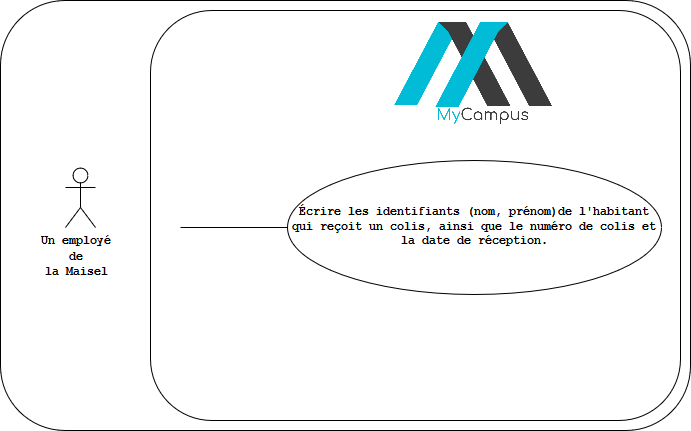
\includegraphics[scale=0.5]{diag_utili.png}
\caption{Diagramme de cas d'utilisation pour un employé de la Maisel}
\end{center}
\end{figure}

\begin{figure}[]
\begin{center}
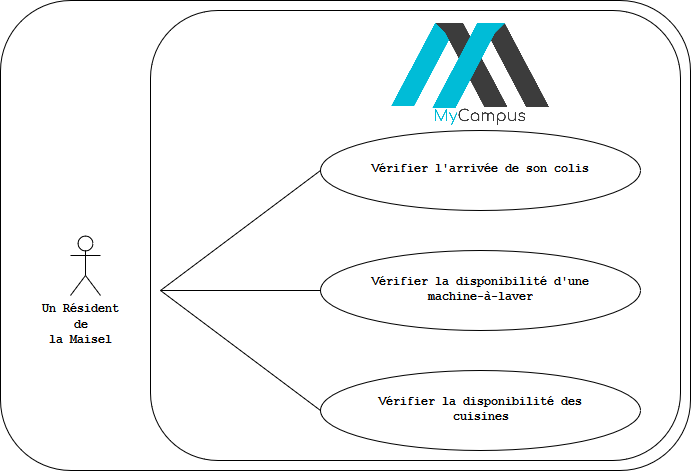
\includegraphics[scale=0.5]{diag_utili2.png}
\caption{Diagramme de cas d'utilisation pour un résident de la Maisel}
\end{center}
\end{figure}

\newpage

\subsubsection{Diagrammes de séquences :}
La plateforme a pour but la réalisation de trois fonctions principales définies précédemment, vous trouvez ci-dessous quatre diagrammes de séquence qui permettent de montrer trois scénarios différents d’un diagramme de cas d’utilisation pour un résident de la Maisel, et l’unique scénario pour un employé de la Maisel.
\bigbreak
\textbf{Scénario 1:}  Un habitant de la Maisel qui demande au chatbot s'il a reçu un colis .
\begin{figure}[h!]
\begin{center}
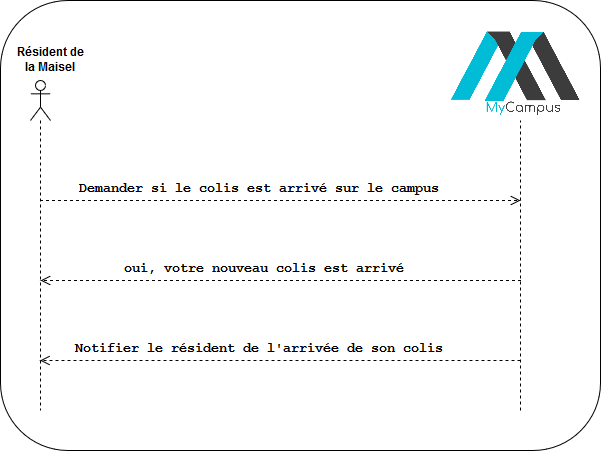
\includegraphics[scale=0.45]{colis.png}
\caption{Diagramme de séquence pour Scénario 1}
\end{center}
\end{figure}


\begin{figure}[h!]
\textbf{Scénario 2:}  Un résident vérifie si une machine à laver est disponible.
\begin{center}
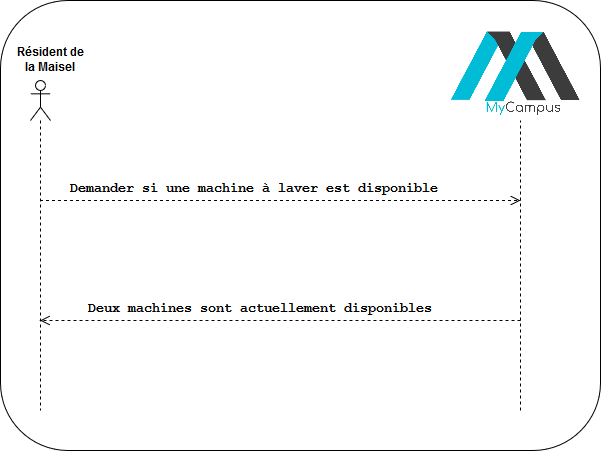
\includegraphics[scale=0.45]{machine.png}
\caption{Diagramme de séquence pour Scénario 2}
\end{center}
\end{figure}


\begin{figure}[]
\textbf{Scénario 3:}  Un résident vérifie si une cuisine est disponible.
\begin{center}
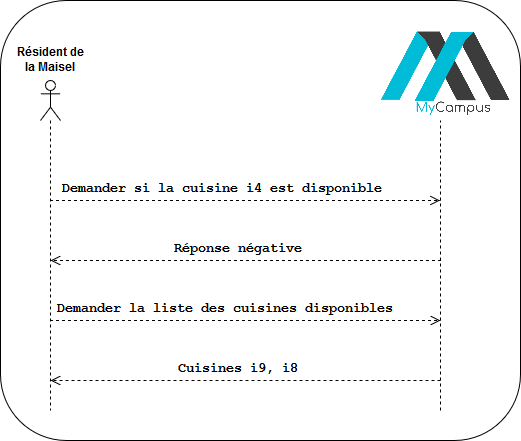
\includegraphics[scale=0.5]{cuisine.png}
\caption{Diagramme de séquence pour Scénario 3}
\end{center}
\end{figure}


\begin{figure}[]
\textbf{Scénario 4:}  Un employé de la Maisel qui décalre un colis arrivé.
\begin{center}
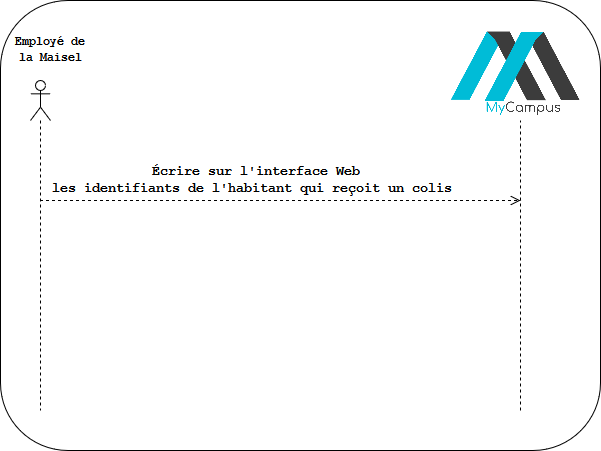
\includegraphics[scale=0.5]{employemaisel.png}
\caption{Diagramme de séquence pour Scénario 4}
\end{center}
\end{figure}


\clearpage

\section{Annexe}
\setcounter{figure}{0}  

\begin{figure}[h!]
\begin{center}
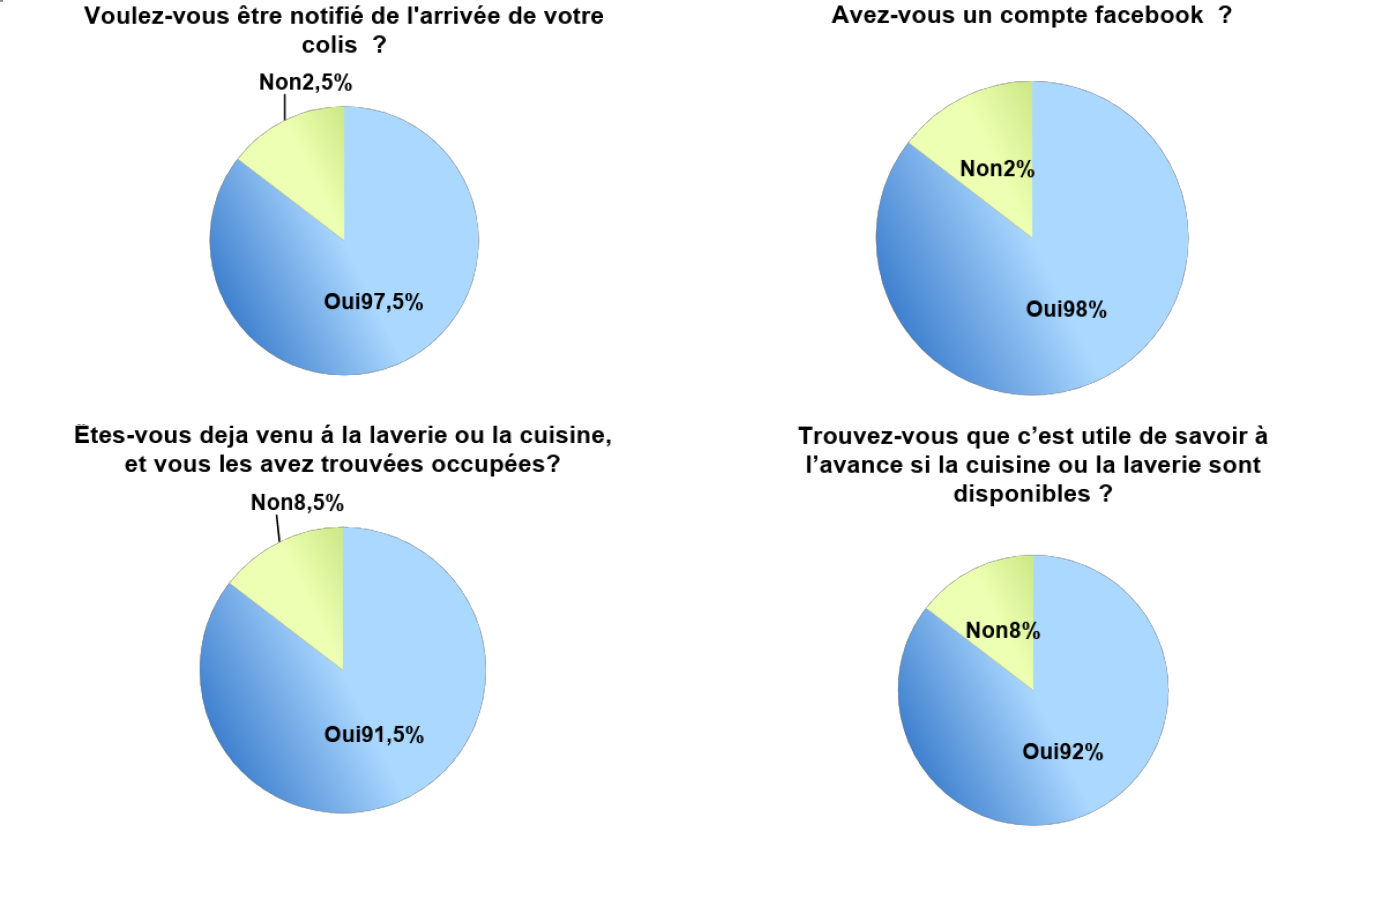
\includegraphics[scale=0.5]{stats.png}
\caption{Mesure de besoin sur la Maisel}
\end{center}
\end{figure}

\begin{figure}[h!]
\begin{center}
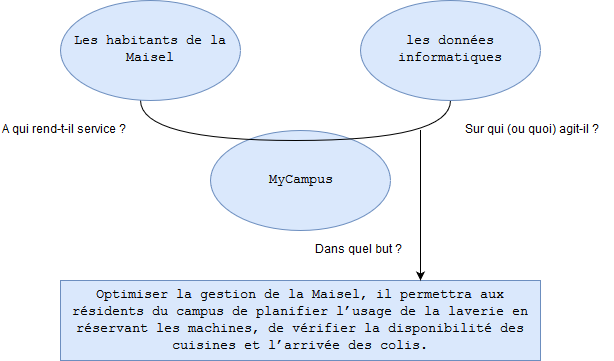
\includegraphics[scale=0.5]{analyse_besoin.png}
\caption{Diagramme d'analyse du besoin}
\end{center}
\end{figure}

\begin{figure}[]
\begin{center}
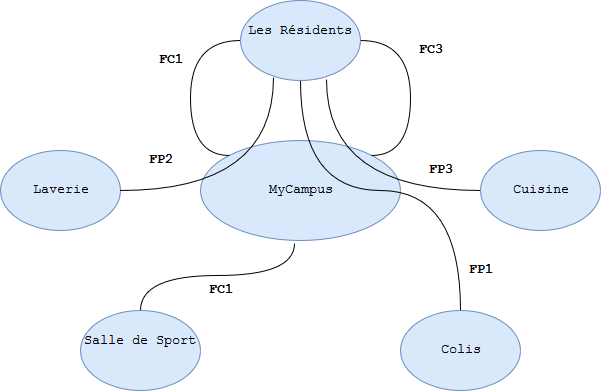
\includegraphics[scale=0.5]{diagramme_pieuvre.png}
\caption{Diagramme pieuvre associé à l'étude de la plateforme MyCampus}
\end{center}
\end{figure}


\end{document}

